At this point, I have identified a set of suitable quality indicators for heart failure at the MUHC and have two \gls{EAF} systems with validated usability and usefulness; a gamified, and a traditional system. I am now ready to estimate how a behavioural intervention focused on intrinsic motivators, gamification, affects adoption, engagement, and effectiveness of an e-A\&F intervention.

The proposed research design is a single center, parallel-arm, actively controlled randomized control trial (\gls{RCT}) of physicians treating heart failure patients at the \gls{MUHC} hospital. Experiment assignement will use a 1:1 ratio. Both systems will present feedback based on the quality measures in objective 1. The trial is planned to last 14 months in total. The RCT design as been chosen as opposed to an impact evaluation to increase the usefulness of the results it generates by aligning more closely with prior evidence in the field. The intervention will be delivered through personalized confidential web-based portal, accessed by navigating to a specific URL on a ward computer or personal device. In this objective, my hypothesis is that there is a difference in adoption of the \gls{EAF} system between the traditionally designed and gamified arm. The null being that there is no difference; same applies for engagement. I consider effectiveness a secondary objective in this trial. The true effect of the systems might be affected by their adaptation, the length of the trial, or what quality measure can be automatically computed. Prior research on system with fewer limit has already shown a positive effects.

\begin{figure}[h]
    \centering
    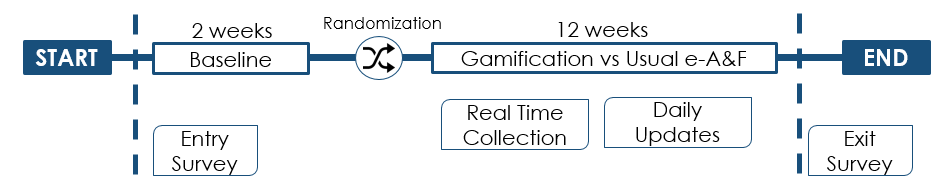
\includegraphics[width=\textwidth]{img/rct_flow.png}
    \caption{Diagram of the RCT process}
    \label{fig:rct_flow}
\end{figure}

\section{Timing, Participants, and Consent}
To participate in this trial, users must be physicians working at the MUHC, have control over the treatment of patients with heart failure, and have worked in the emergency department (ED) or in the intensive care unit (ICU) for at least 10 weeks\footnote{Baseline assessment + 2 months}. This will include attending physicians, medical residents, and fellow. Participants will be followed for a maximum of 12 weeks after the mandatory 2 weeks baseline assessment. The choice of 12 weeks was made by balancing feasibility with the need for participants and for enough follow-up to measure retention. No recruitment will be attempted in the last 2 months of the trial. Recruitment will be made by informing the different department, with recruitment material, and with a local champion.

% Consent Process
Since only secondary patient data is used, and since it is used as part of the care process, a blanket consent will be requested from the direction of professional services. Informed consent will be required from each participant and participants can stop using either intervention at any time. Participants will not be allowed to switch arm. If participants inform us of their desire to stop using the interventions, an exit survey will be sent to them.

\section{Data Collection}
No \textit{clinical} data will be captured specifically for this project. Patient data is only used to create provider-level feedback. Providers will be able to see nominative data for themselves and their own patients. Both systems will automate indicator processing from patient data as described in the "data source" section. Simple randomization will be performed by the tool after a user fill the entry questionnaire. Both system will perform real time data collection as participants use them. Data will be logged into a secured database, assigned to the anonymous ID of the participant. Participants quality measures will be confidential and will not be shared. All analysis will be performed on participants' anonymous IDs. Participant data will be stored for a duration of 7 years, an any identifier will be removed as soon as all data is collected for a participant. The data analyst will be blinded to treatment assignment, but the participants cannot.

\section{Measures and Outcomes}

Participants will need to fill an entry questionnaire on their first connection. The questions will include basic demographics (10 year age groups, gender, years of practice, attending/resident/fellow), whether they are aware of following any explicit guidelines, and if they tried any auditing of their practice. An exit questionnaire will be sent to participants at the end of the trial. It will be the System Usability Scale (SUS), a validated and widely used 10-question tool for measuring perception of usability.\cite{united2006research}

% Define and describe how they are collected and at which frequency.
I will use the HEART framework to operationalize the criteria for the third objective. This framework for user-centred metrics addresses previous deficiencies in measuring user experience quality, and providing actionable data. In addition to the next table, secondary metrics will be collected for exploratory purposes: 1) Useless clicks, 2) time on site, 3) number of 90-day with at least one non-trivial action.\cite{rodden2010measuring}

\begingroup
\setlength{\tabcolsep}{8pt} % Default value: 6pt
\renewcommand{\arraystretch}{1.5} % Default value: 1
\small
\begin{table}[h!]
\begin{tabular}{l|l|l}
\textbf{Measure}       & \textbf{Metric}                  & \textbf{Meaning}                           \\
\hline                                                                                                    
\textbf{Adoption}      & any 2 login, except registration & how many new users start using a product   \\
\textbf{Retention}     & 90-day periods with ≥ 1 login    & how many of the users are still present    \\
\textbf{Engagement}    & login per 90-day period          & user’s level of involvement with a product \\
\textbf{Effectiveness} & estimate for quality indicators  & how much a user accomplished                                       
\end{tabular}
\end{table}
\endgroup

\section{Statistical Plan}\footnote{Made following "Guidelines for the content of statistical analysis plans in clinical trials. Gamble 2017"}
% Descriptive statistics
Descriptive statistics on the variables in the entry survey will be summarized by randomization group. Categorical data will be summarised by numbers and percentages, while continuous by mean and standard deviation. Standardized difference will be presented to assess the success of randomization but no statistical test will be used. A CONSORT diagram will be presented to describe patient flow.

% Analysis
The intention-to-treat population will include all randomised patients, regardless of their eligibility, according to the treatment they where randomized to receive. Final analysis will be performed for all data at once, at the end of the trial. All applicable statistical tests will be 2-sided and will be performed using a 5\% significance level, including confidence intervals. The unadjusted analysis will be performed by testing for the overlap of 95\% confidence intervals for all main outcomes: proportions for adoption, means for retention, means for engagement (see Measures for units). Analysis of the secondary outcome, change in effectiveness, will also use overlap of CI, but the estimate compared is the average difference in scores between the start and end of the trial. Quality measures in patients which could not be computed for more than half of the trials will not be disregarded. Since data can only be missing on the exit survey, and since this survey is only used for explanatory purposes, a complete case analysis will be used. A sub-group analysis will be performed separating attending physicians, residents, and fellow. Also, the differences for each quality measure, between arm, will be presented in a forest plot styled visualization. Any feedback of adverse event will be reported. A sensitivity analysis will be performed on the effect of not removing quality indicators.

\section{Sample Size}
A sample size calculation is provided, but the population of potential candidates is of finite size. I will try to recruit as mainly provider as I can regardless of the associated estimated size. Normally, I would like to provide an estimate for both main outcomes, adoption and engagement, but since adoption is rarely reported, only an estimate for engagement as a comparison of means will be provided. The calculation will make use of a mixed Bayesian/likelihood procedure assuming known precision/variance to compute an average length criterion. This procedure given priors for the common precision, the desired average length of the posterior credible interval between the two unknown means, and a desired coverage probability (here 0.95) estimates the required sample size.

No suitable data was found from the field of \gls{EAF}, but I will use an example from the study of a gamified peer-to-peer trading service. I find this research suitable since 1) they collected at least a year of data, 2) it is also a high skill situation, 3) user can also face poor performance, 4) it is also a web-portal.\cite{hamari2017badges} The important data from the study is an effect of gamification on mean occasion visited of 0.27 [0.19, 0.34].\footnote{Results were obtained using \cite{looyestyn2017does}} It also provides basic statistics on the page view distribution between the two group. The tool used for the calculation is the SampleSizeMeans R package.\cite{joseph1997bayesian}

There are two modification, first there base page views are much too high to suit this context. Based on the potential quality measures and the rate of patients seen, I would expect around 1 login per 90 days for the base system. Data from the study will be scaled to this number. Also, I computed two sample size, one conservative and one optimistic. Given the original study was a trading tool, I would expect much more variation in views than in an \gls{EAF}. Using the variance from the study (conservative estimate), I get a sample size of 2714. Limiting the standard deviation to more temperate values of 0.5 for the control and 0.7 for the experiment, I get a sample size of 156. See appendix B for exact code. These numbers do not take into account attrition or participation rates. It is also difficult to put a measure on a "clinical meaningfulness threshold" of engagement. Based on an average of the last 5 years, we would need 58\% participation to get at least 156 users.

% Why not :
%
% 1- Crossover
%    Cross-over might not be appropriate due to concerns of carryover effects.
% 2- Stop Rule
%    Difficulty of finding good prior estimate of many measures, and to put a clinically significant
%    threshold on them.
% 3- Why not using a complier average causal effect (CACE) analysis.
%    ???
% 4- How to adjust for people who have diff end - start based on 2 mths vs 12 mths. Less opportunity
%    ??? RCT doesn't care?
% 5- How is power measured in this context?